% Options for packages loaded elsewhere
\PassOptionsToPackage{unicode}{hyperref}
\PassOptionsToPackage{hyphens}{url}
\PassOptionsToPackage{dvipsnames,svgnames,x11names}{xcolor}
%
\documentclass[
  letterpaper,
  DIV=11,
  numbers=noendperiod]{scrartcl}

\usepackage{amsmath,amssymb}
\usepackage{iftex}
\ifPDFTeX
  \usepackage[T1]{fontenc}
  \usepackage[utf8]{inputenc}
  \usepackage{textcomp} % provide euro and other symbols
\else % if luatex or xetex
  \usepackage{unicode-math}
  \defaultfontfeatures{Scale=MatchLowercase}
  \defaultfontfeatures[\rmfamily]{Ligatures=TeX,Scale=1}
\fi
\usepackage{lmodern}
\ifPDFTeX\else  
    % xetex/luatex font selection
\fi
% Use upquote if available, for straight quotes in verbatim environments
\IfFileExists{upquote.sty}{\usepackage{upquote}}{}
\IfFileExists{microtype.sty}{% use microtype if available
  \usepackage[]{microtype}
  \UseMicrotypeSet[protrusion]{basicmath} % disable protrusion for tt fonts
}{}
\makeatletter
\@ifundefined{KOMAClassName}{% if non-KOMA class
  \IfFileExists{parskip.sty}{%
    \usepackage{parskip}
  }{% else
    \setlength{\parindent}{0pt}
    \setlength{\parskip}{6pt plus 2pt minus 1pt}}
}{% if KOMA class
  \KOMAoptions{parskip=half}}
\makeatother
\usepackage{xcolor}
\setlength{\emergencystretch}{3em} % prevent overfull lines
\setcounter{secnumdepth}{5}
% Make \paragraph and \subparagraph free-standing
\makeatletter
\ifx\paragraph\undefined\else
  \let\oldparagraph\paragraph
  \renewcommand{\paragraph}{
    \@ifstar
      \xxxParagraphStar
      \xxxParagraphNoStar
  }
  \newcommand{\xxxParagraphStar}[1]{\oldparagraph*{#1}\mbox{}}
  \newcommand{\xxxParagraphNoStar}[1]{\oldparagraph{#1}\mbox{}}
\fi
\ifx\subparagraph\undefined\else
  \let\oldsubparagraph\subparagraph
  \renewcommand{\subparagraph}{
    \@ifstar
      \xxxSubParagraphStar
      \xxxSubParagraphNoStar
  }
  \newcommand{\xxxSubParagraphStar}[1]{\oldsubparagraph*{#1}\mbox{}}
  \newcommand{\xxxSubParagraphNoStar}[1]{\oldsubparagraph{#1}\mbox{}}
\fi
\makeatother


\providecommand{\tightlist}{%
  \setlength{\itemsep}{0pt}\setlength{\parskip}{0pt}}\usepackage{longtable,booktabs,array}
\usepackage{calc} % for calculating minipage widths
% Correct order of tables after \paragraph or \subparagraph
\usepackage{etoolbox}
\makeatletter
\patchcmd\longtable{\par}{\if@noskipsec\mbox{}\fi\par}{}{}
\makeatother
% Allow footnotes in longtable head/foot
\IfFileExists{footnotehyper.sty}{\usepackage{footnotehyper}}{\usepackage{footnote}}
\makesavenoteenv{longtable}
\usepackage{graphicx}
\makeatletter
\def\maxwidth{\ifdim\Gin@nat@width>\linewidth\linewidth\else\Gin@nat@width\fi}
\def\maxheight{\ifdim\Gin@nat@height>\textheight\textheight\else\Gin@nat@height\fi}
\makeatother
% Scale images if necessary, so that they will not overflow the page
% margins by default, and it is still possible to overwrite the defaults
% using explicit options in \includegraphics[width, height, ...]{}
\setkeys{Gin}{width=\maxwidth,height=\maxheight,keepaspectratio}
% Set default figure placement to htbp
\makeatletter
\def\fps@figure{htbp}
\makeatother
% definitions for citeproc citations
\NewDocumentCommand\citeproctext{}{}
\NewDocumentCommand\citeproc{mm}{%
  \begingroup\def\citeproctext{#2}\cite{#1}\endgroup}
\makeatletter
 % allow citations to break across lines
 \let\@cite@ofmt\@firstofone
 % avoid brackets around text for \cite:
 \def\@biblabel#1{}
 \def\@cite#1#2{{#1\if@tempswa , #2\fi}}
\makeatother
\newlength{\cslhangindent}
\setlength{\cslhangindent}{1.5em}
\newlength{\csllabelwidth}
\setlength{\csllabelwidth}{3em}
\newenvironment{CSLReferences}[2] % #1 hanging-indent, #2 entry-spacing
 {\begin{list}{}{%
  \setlength{\itemindent}{0pt}
  \setlength{\leftmargin}{0pt}
  \setlength{\parsep}{0pt}
  % turn on hanging indent if param 1 is 1
  \ifodd #1
   \setlength{\leftmargin}{\cslhangindent}
   \setlength{\itemindent}{-1\cslhangindent}
  \fi
  % set entry spacing
  \setlength{\itemsep}{#2\baselineskip}}}
 {\end{list}}
\usepackage{calc}
\newcommand{\CSLBlock}[1]{\hfill\break\parbox[t]{\linewidth}{\strut\ignorespaces#1\strut}}
\newcommand{\CSLLeftMargin}[1]{\parbox[t]{\csllabelwidth}{\strut#1\strut}}
\newcommand{\CSLRightInline}[1]{\parbox[t]{\linewidth - \csllabelwidth}{\strut#1\strut}}
\newcommand{\CSLIndent}[1]{\hspace{\cslhangindent}#1}

\KOMAoption{captions}{tableheading}
\makeatletter
\@ifpackageloaded{tcolorbox}{}{\usepackage[skins,breakable]{tcolorbox}}
\@ifpackageloaded{fontawesome5}{}{\usepackage{fontawesome5}}
\definecolor{quarto-callout-color}{HTML}{909090}
\definecolor{quarto-callout-note-color}{HTML}{0758E5}
\definecolor{quarto-callout-important-color}{HTML}{CC1914}
\definecolor{quarto-callout-warning-color}{HTML}{EB9113}
\definecolor{quarto-callout-tip-color}{HTML}{00A047}
\definecolor{quarto-callout-caution-color}{HTML}{FC5300}
\definecolor{quarto-callout-color-frame}{HTML}{acacac}
\definecolor{quarto-callout-note-color-frame}{HTML}{4582ec}
\definecolor{quarto-callout-important-color-frame}{HTML}{d9534f}
\definecolor{quarto-callout-warning-color-frame}{HTML}{f0ad4e}
\definecolor{quarto-callout-tip-color-frame}{HTML}{02b875}
\definecolor{quarto-callout-caution-color-frame}{HTML}{fd7e14}
\makeatother
\makeatletter
\@ifpackageloaded{caption}{}{\usepackage{caption}}
\AtBeginDocument{%
\ifdefined\contentsname
  \renewcommand*\contentsname{Table of contents}
\else
  \newcommand\contentsname{Table of contents}
\fi
\ifdefined\listfigurename
  \renewcommand*\listfigurename{List of Figures}
\else
  \newcommand\listfigurename{List of Figures}
\fi
\ifdefined\listtablename
  \renewcommand*\listtablename{List of Tables}
\else
  \newcommand\listtablename{List of Tables}
\fi
\ifdefined\figurename
  \renewcommand*\figurename{Figure}
\else
  \newcommand\figurename{Figure}
\fi
\ifdefined\tablename
  \renewcommand*\tablename{Table}
\else
  \newcommand\tablename{Table}
\fi
}
\@ifpackageloaded{float}{}{\usepackage{float}}
\floatstyle{ruled}
\@ifundefined{c@chapter}{\newfloat{codelisting}{h}{lop}}{\newfloat{codelisting}{h}{lop}[chapter]}
\floatname{codelisting}{Listing}
\newcommand*\listoflistings{\listof{codelisting}{List of Listings}}
\makeatother
\makeatletter
\makeatother
\makeatletter
\@ifpackageloaded{caption}{}{\usepackage{caption}}
\@ifpackageloaded{subcaption}{}{\usepackage{subcaption}}
\makeatother
\ifLuaTeX
  \usepackage{selnolig}  % disable illegal ligatures
\fi
\usepackage{bookmark}

\IfFileExists{xurl.sty}{\usepackage{xurl}}{} % add URL line breaks if available
\urlstyle{same} % disable monospaced font for URLs
\hypersetup{
  pdftitle={Extreme Weather Events Data: Analysis},
  pdfauthor={Emmanuel Guizar Rosales},
  colorlinks=true,
  linkcolor={blue},
  filecolor={Maroon},
  citecolor={Blue},
  urlcolor={Blue},
  pdfcreator={LaTeX via pandoc}}

\title{Extreme Weather Events Data: Analysis}
\author{Emmanuel Guizar Rosales}
\date{last rendered on: Aug 16, 2024}

\begin{document}
\maketitle

\renewcommand*\contentsname{Table of contents}
{
\hypersetup{linkcolor=}
\setcounter{tocdepth}{5}
\tableofcontents
}
\section{Purpose \& Rationale}\label{purpose-rationale}

As outlined in the Registered Report, we will assess the number of
extreme weather episodes recorded in each participant's county of
residence within the 30 days prior to study completion. Regarding the
time window during which we plan to conduct the study, we aim for
maximizing the likelihood of capturing suitable variability in the
exposure to extreme weather episodes with notable geographic
variability. To this end, we analyzed records of extreme weather
episodes over the last ten years.

\section{Filter Data}\label{filter-data}

We filter the storm events data for the specific years, months, and
extreme weather event types we are interested in. We filter for all
years from 2014 to 2023 (as data are not complete for the year 2024
yet), we highlight the month of July, and we focus on those types of
extreme weather events that are predicted to increase in frequency and
severity due to climate change (IPCC 2023): Excessive Heat, Drought,
Wildfire, Flash Flood, Coastal Flood, Strong Wind, Hail, and Tornado.

\section{Analysis}\label{analysis}

Analyzing the seasonal distribution of extreme weather episodes,
Figure~\ref{fig-p.hist} shows that July consistently shows a high number
of extreme weather episodes over the last ten years. Additionally,
Figure~\ref{fig-p.map_bin} indicates that withing the month of July,
these extreme weather episodes also display a high geographical
variability.

\begin{figure}[h]

\centering{

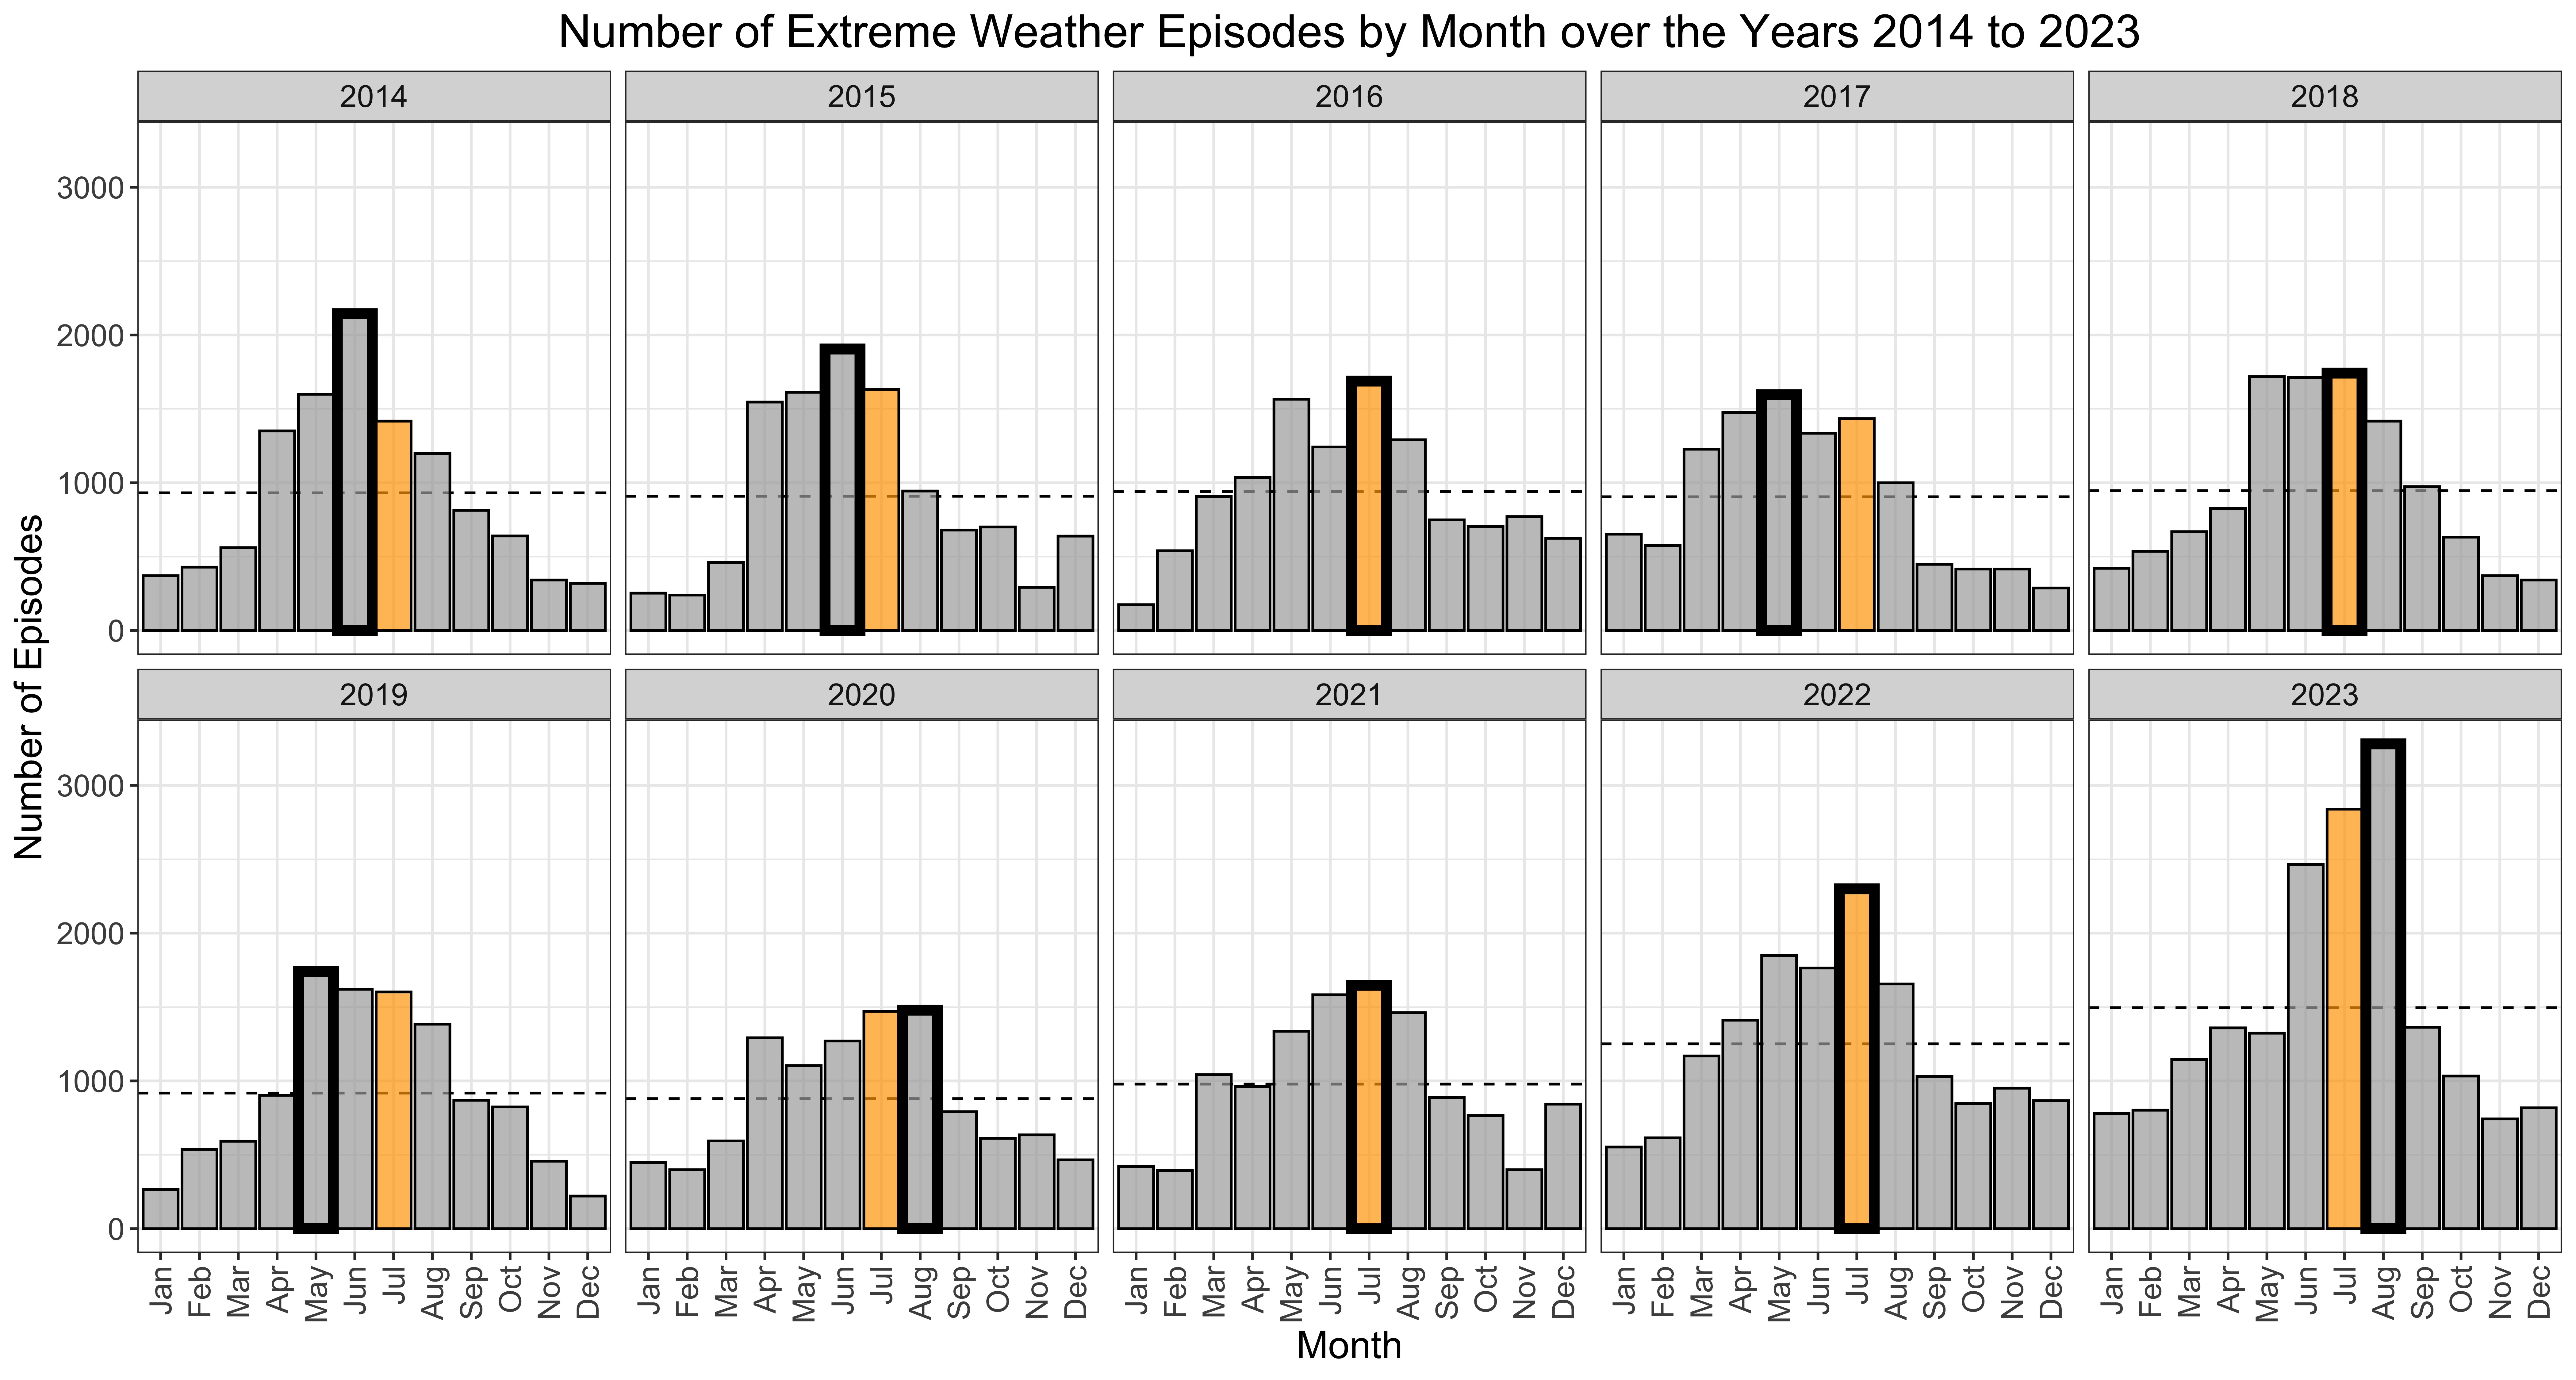
\includegraphics{../images/histogramSeasonalDistribution.jpeg}

}

\caption{\label{fig-p.hist}Histograms showing the number of extreme
weather episodes by month from 2014 to 2023. The dashed horizontal line
indicates the mean number of extreme weather episodes in each year. The
thick-bordered bar marks the month with the most extreme weather events
each year. The orange bar represents July. July had the most extreme
weather events in 4 out of 10 years, and in another 4 years, it was
right before or after the peak month. Only episodes that included at
least one of the following event types were considered: excessive heat,
drought, wildfire, flash flood, coastal flood, strong wind, hail,
tornado.}

\end{figure}%

\begin{figure}[h]

\centering{

\includegraphics{../images/mapGeographicalDistribution_bin.jpeg}

}

\caption{\label{fig-p.map_bin}Maps displaying the geographical
distribution of the occurrence of at least one extreme weather episode
in July over the years 2014 to 2023. Only episodes that included at
least one of the following event types were considered: excessive heat,
drought, wildfire, flash flood, coastal flood, strong wind, hail,
tornado.}

\end{figure}%

While Figure~\ref{fig-p.map_bin} visualizes the occurrence of at least
one extreme weather episode in July for each county and year (binary
variable), Figure~\ref{fig-p.hist_cont} displays the actual number of
such episodes (continuous). The vast majority of counties were exposed
to few episodes, indicating that most of the variability is due to
whether an extreme weather episode occurred at all or not. This is
further supported by Figure~\ref{fig-p.map_cont} showing histograms for
the number of extreme weather episodes in July over the past ten years.
Most counties reported either zero or one extreme weather episode in
July, and the ratio of counties experiencing no episodes to counties
experiencing at least one episode seems to gradually approach 1:1. In
July 2023, for instance, this ratio reached 1.02, with 50.43\% of
counties being exposed to zero and 49.57\% of counties being exposed to
at least one extreme weather episode.

\begin{figure}[h]

\centering{

\includegraphics{../images/mapGeographicalDistribution_cont.jpeg}

}

\caption{\label{fig-p.map_cont}Maps displaying the geographical
distribution of the raw number of extreme weather episodes in July over
the years 2014 to 2023. The color palette indicates numbers greater than
zero, and white represent a count of zero episodes.}

\end{figure}%

\begin{figure}[h]

\centering{

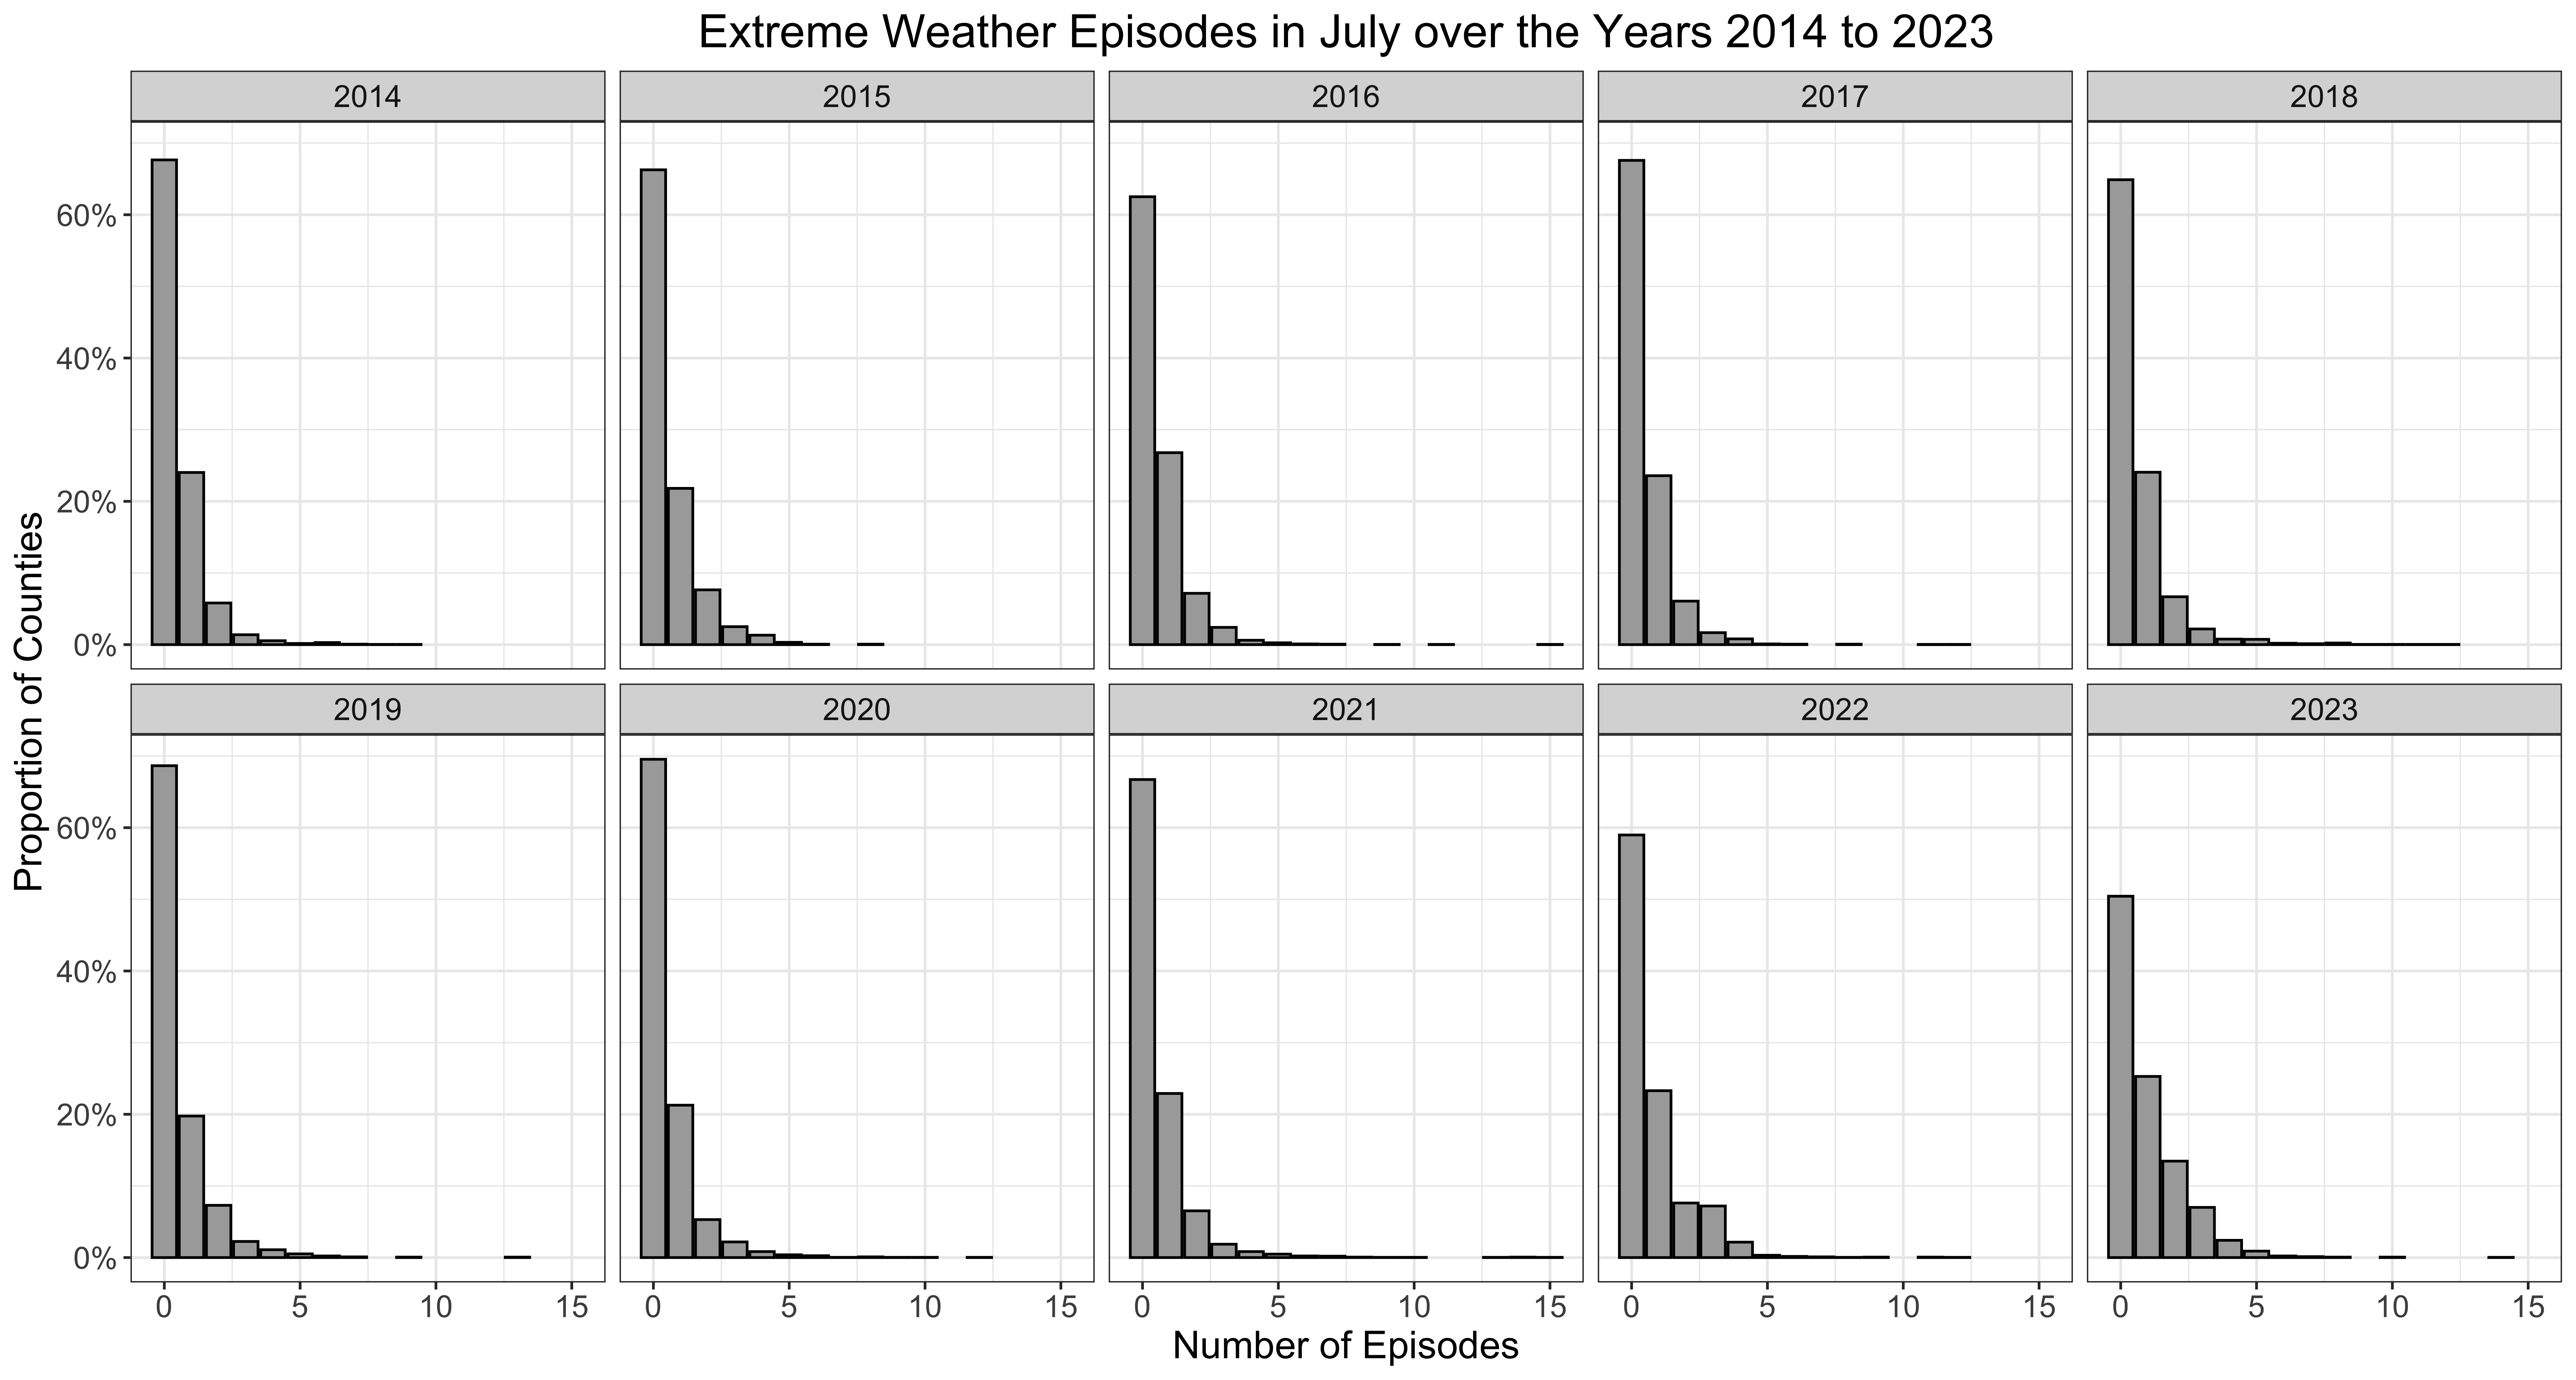
\includegraphics{../images/frequencyDistribution_cont.jpeg}

}

\caption{\label{fig-p.hist_cont}Histograms displaying the distribution
of the raw number of extreme weather episodes in July over the years
2014 to 2023. For each number of episodes on the x-axis, the y-axis
shows the proportion of counties that recorded this number of episodes.}

\end{figure}%

Finally, as reported in the analysis plan and the design table, we plan
to run a set of additional analyses regarding hypotheses
H\textsubscript{2} and H\textsubscript{3}, in which we will test the
sensitivity of results to the time period prior to study completion used
to assess extreme weather exposure. Regarding H\textsubscript{2}, we
will estimate the two-way interaction effect of political affiliation
and extreme weather exposure on ΔDuration for different time periods
from 30 days to 360 days in increments of 30 days. Similarly for
H\textsubscript{3}, we will estimate the three-way interaction effect of
political affiliation, extreme weather exposure, and attribution of
extreme weather events to climate change on ΔDuration for the same time
periods. We will visualize results of these additional analyses by
plotting the two-way (or three-way) interaction regression coefficients
as points surrounded by their 95\%-CI on the y-axis and the 12 time
periods on the x-axis, as displayed in Figure~\ref{fig-p.sensitivity}
with simulated data. Based on previous research (Konisky, Hughes, and
Kaylor 2016), we expect that the estimated effects will decay as the
number of days prior to study completion used to assess the occurrence
of extreme weather episodes increases.

\begin{figure}[h]

\centering{

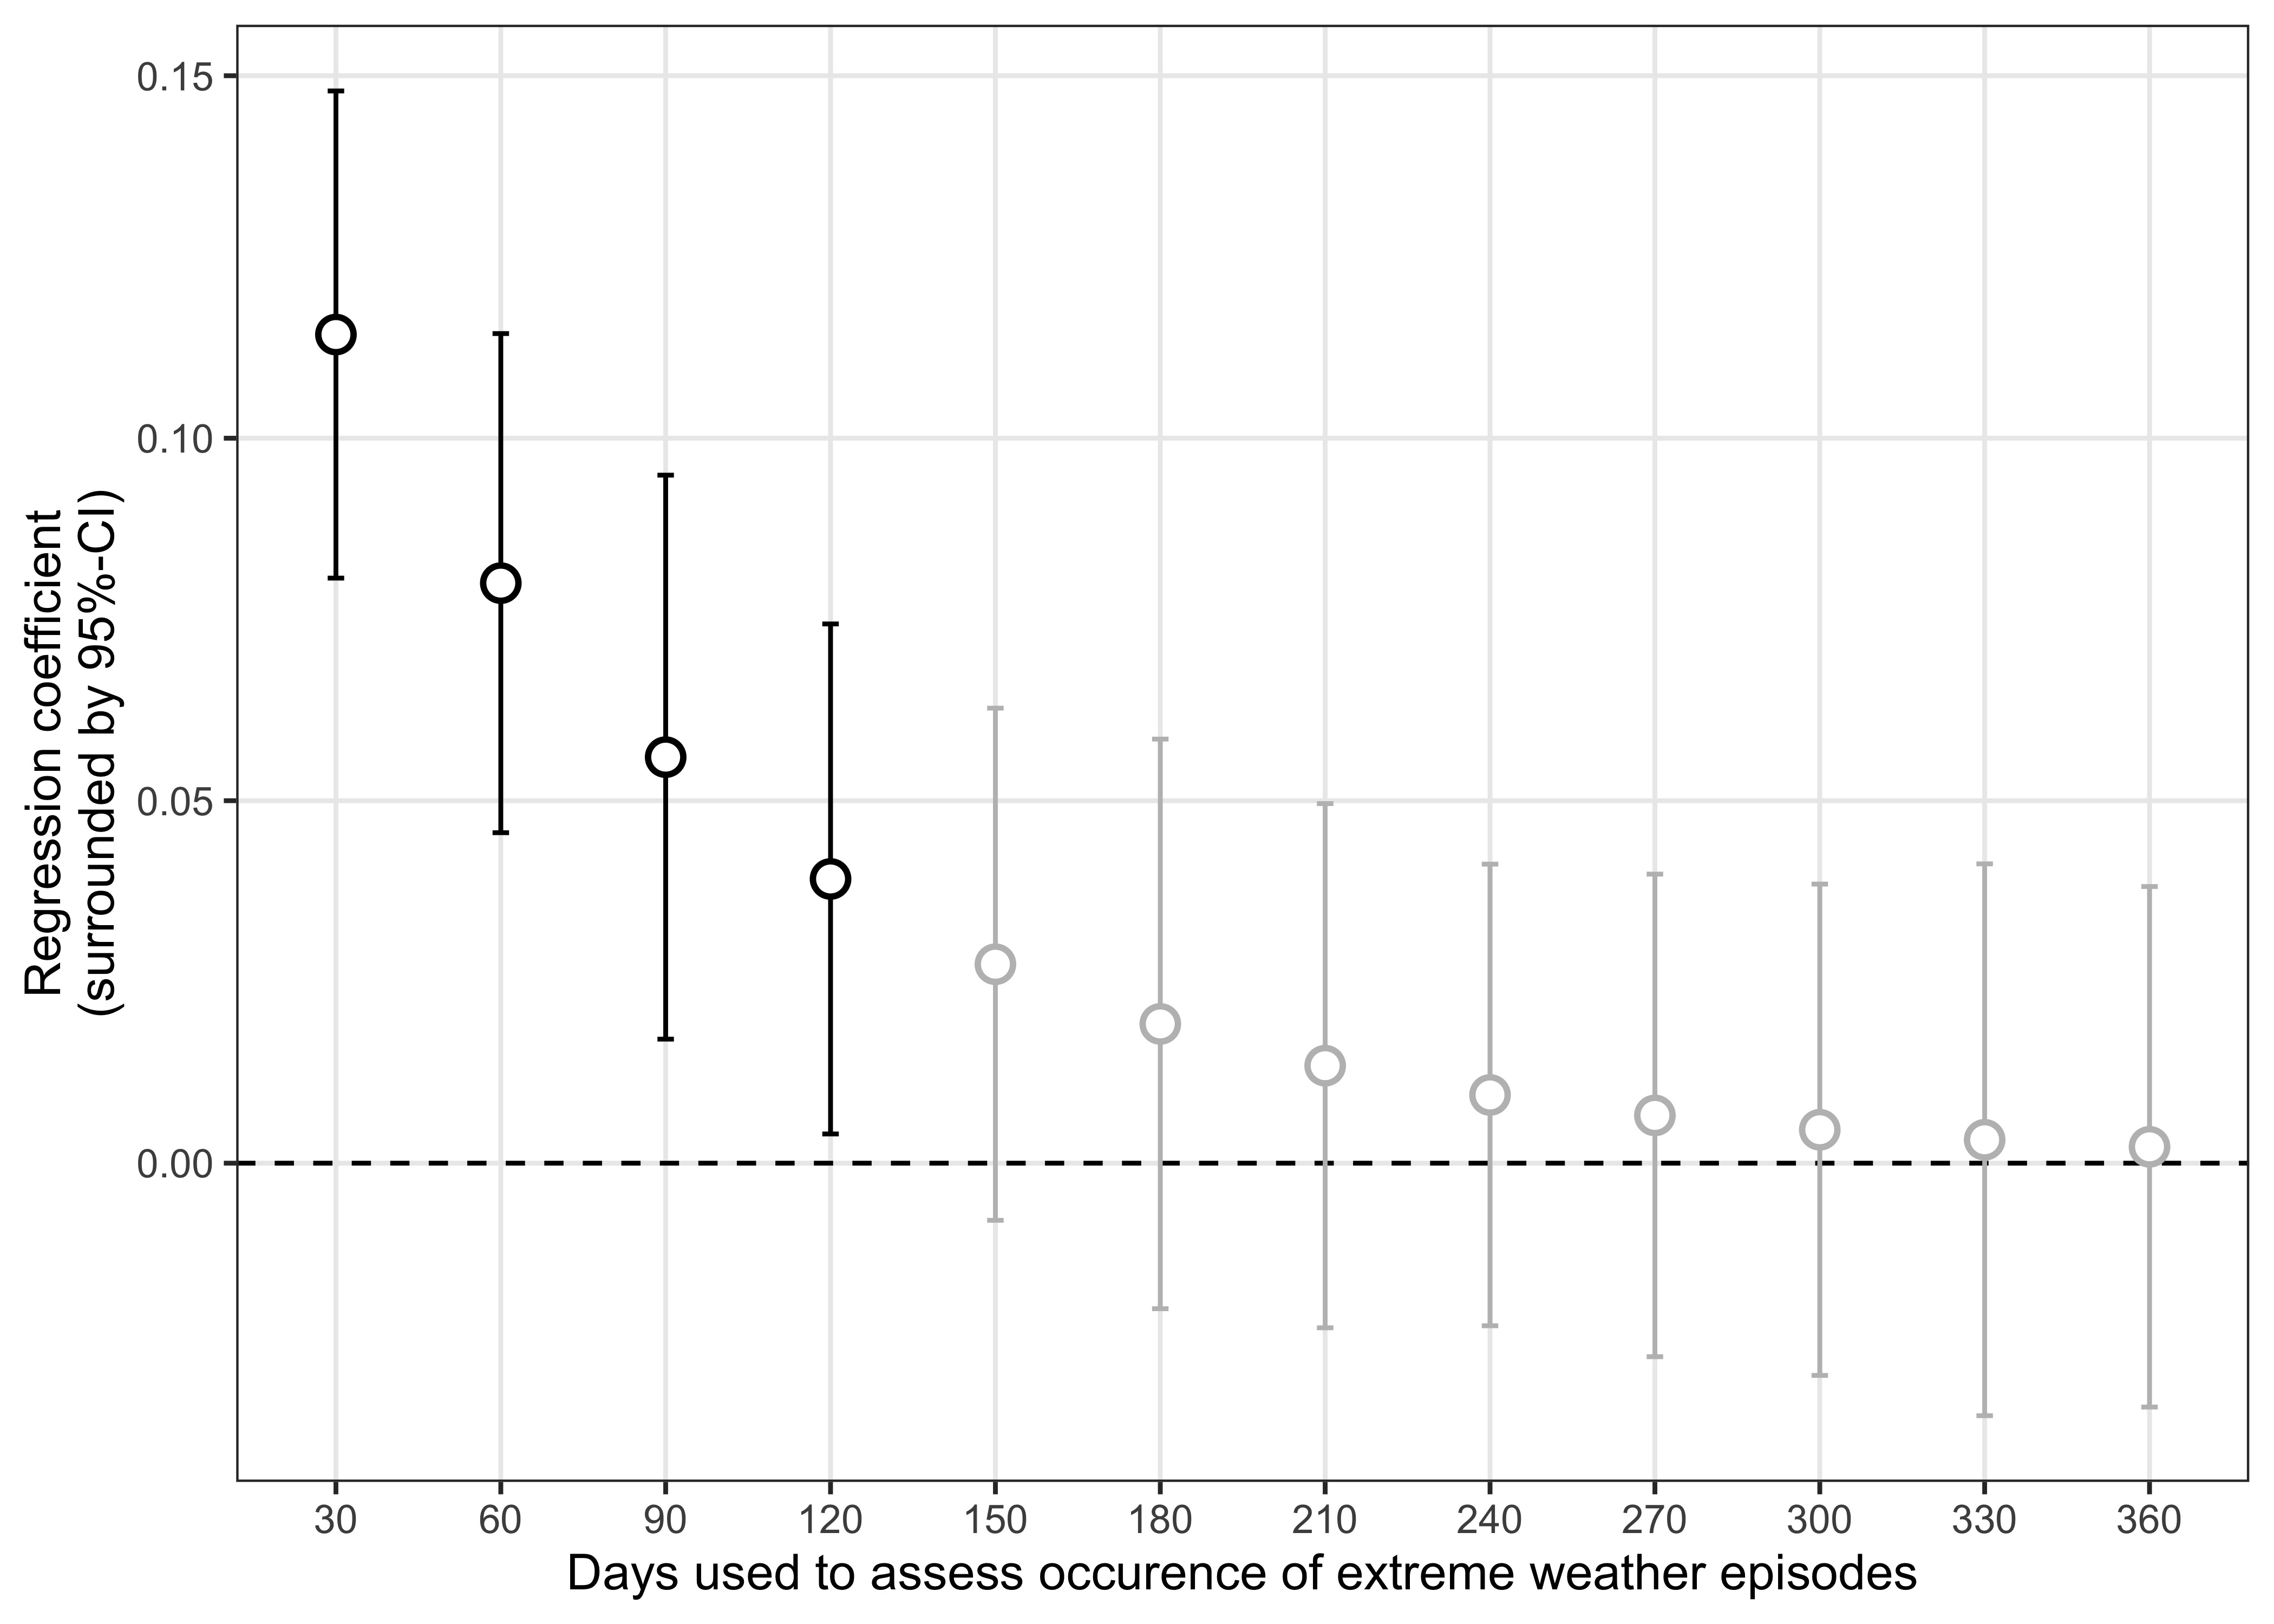
\includegraphics{../images/sensitivityAnalyses_simulation.jpeg}

}

\caption{\label{fig-p.sensitivity}Simulated regression coefficients of
interaction effects for different number of days prior to study
completion used to assess the occurrence of extreme weather episodes.
Point estimates are surrounded by their 95\% confidence intervals. The
dashed line represents the absence of an interaction effect (regression
coefficient of zero). Significance of regression coefficients is
color-coded, with black indicating regression coefficients significantly
different from zero, and grey indicating no significant difference from
zero.}

\end{figure}%

\section{Conclusion}\label{conclusion}

Our analyses indicate that July consistently shows a high number of
extreme whether episodes with notable geographic variability
(Figure~\ref{fig-p.hist} and Figure~\ref{fig-p.map_bin}). Therefore, to
maximize the likelihood of capturing suitable variability in exposure to
extreme weather episodes, we plan to conduct our study at the beginning
of August, ensuring that the 30-day period prior to study completion
falls within July. Moreover, the main source of variability in exposure
to extreme weather episodes in July is due to whether at least one
episode occurred or not (Figure~\ref{fig-p.hist_cont} and
Figure~\ref{fig-p.hist_cont}). Thus, our main analyses will focus on
whether a participant was exposed to at least one extreme weather
episode in the 30 days prior to study completion, treated as a binary
variable. In additional analyses, we will test the sensitivity of our
results to different time periods used to assess extreme weather
exposure prior to study completion.

\begin{tcolorbox}[enhanced jigsaw, left=2mm, colback=white, leftrule=.75mm, opacityback=0, breakable, toprule=.15mm, arc=.35mm, bottomrule=.15mm, rightrule=.15mm, colframe=quarto-callout-note-color-frame]
\begin{minipage}[t]{5.5mm}
\textcolor{quarto-callout-note-color}{\faInfo}
\end{minipage}%
\begin{minipage}[t]{\textwidth - 5.5mm}

\vspace{-3mm}\textbf{Expand for Session Info}\vspace{3mm}

\end{minipage}%
\end{tcolorbox}

\section*{References}\label{references}
\addcontentsline{toc}{section}{References}

\phantomsection\label{refs}
\begin{CSLReferences}{1}{0}
\bibitem[\citeproctext]{ref-ipcc2023}
IPCC, ed. 2023. {``Weather and Climate Extreme Events in a Changing
Climate.''} In, 1513--1766. Cambridge: Cambridge University Press.
\url{https://doi.org/10.1017/9781009157896.013}.

\bibitem[\citeproctext]{ref-konisky2016}
Konisky, David M., Llewelyn Hughes, and Charles H. Kaylor. 2016.
{``Extreme Weather Events and Climate Change Concern.''} \emph{Climatic
Change} 134 (4): 533--47.
\url{https://doi.org/10.1007/s10584-015-1555-3}.

\end{CSLReferences}



\end{document}
